\makeheading{Lecture 8 | 2020-09-30}
The example done in R is included in the next page.
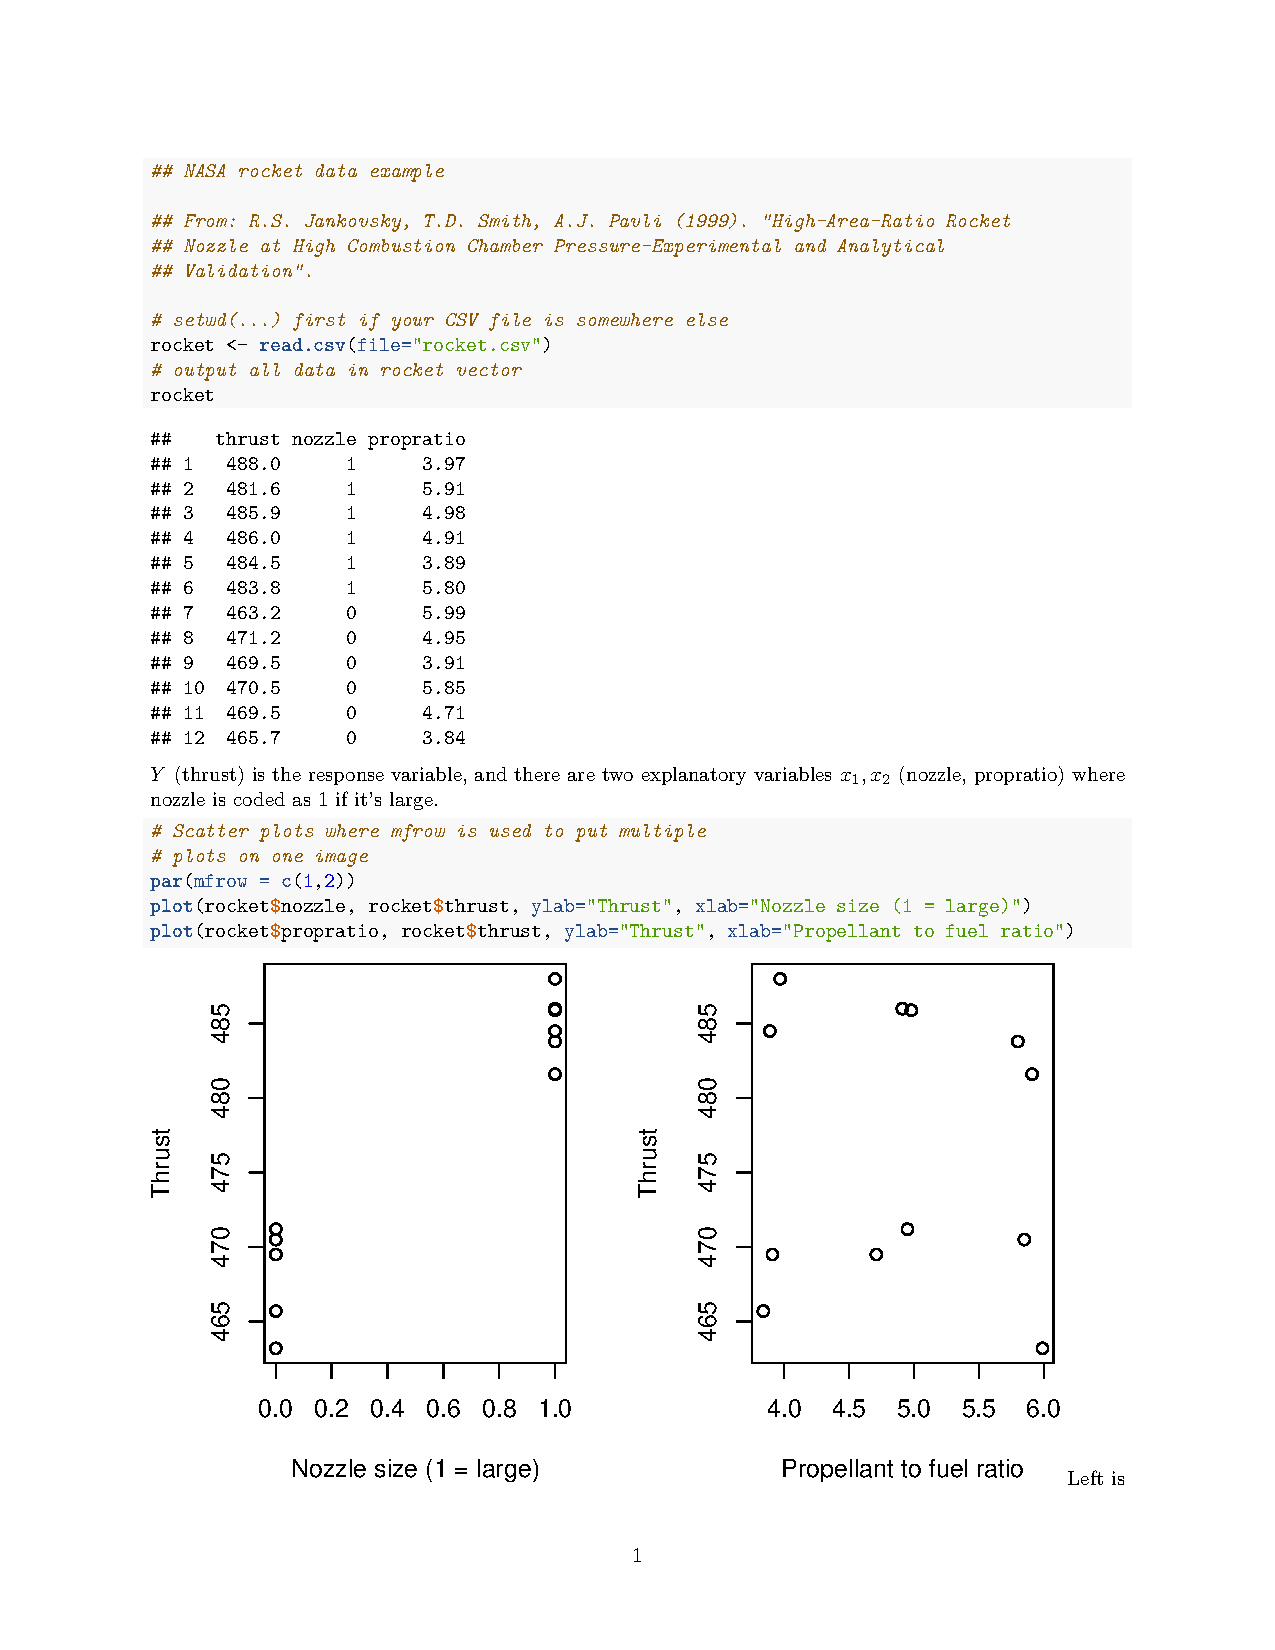
\includepdf[pages=-]{rocket-MLR.pdf}

Handling categorical variables: when there are explanatory
variables with values that fall into one of
several categories.
\begin{itemize}
    \item e.g.\ nozzle large/small, if just binary,
          code as 1 and 0
    \item ordered small, medium, large or not
          red, blue, green
\end{itemize}
\underline{Approach}: can convert to indicator variables
or treat as numerical if it makes sense to do so.

\underline{Example}: Coffee Quality Institute (2018)

Extract a few variables:
\begin{table}[H]
    \centering
    \begin{tabularx}{0.7\linewidth}{@{}YYY@{}}
          & Acidity & Method             \\
        \midrule
        1 & 8.7     & Washed-wet         \\
        2 & 8.3     & Washed-wet         \\
        3 & 8.2     & Natural-dry        \\
        4 & 8.4     & Semi-washed/pulped
    \end{tabularx}
\end{table}
Flavour (response)

How to set up $ X $? For example,
\[ x_{i2}=\begin{cases*}
        0 & dry\\
        1 & semi\\
        2 & wet
    \end{cases*} \]
Not generally appropriate unless we think
a response is linear according to this scheme.

More flexible approach: indicator/dummy variables
\[ x_{i2}=\begin{cases*}
        1 & semi\\
        0 & otherwise
    \end{cases*},\quad
    x_{i3}=\begin{cases*}
        1 & wet\\
        0 & otherwise
    \end{cases*} \]
Therefore,
\[ X=\begin{bmatrix}
        1 & 8.7 & 0 & 1 \\
        1 & 8.3 & 0 & 1 \\
        1 & 8.2 & 0 & 0 \\
        1 & 8.4 & 1 & 0 \\
    \end{bmatrix} \]
Why not $ x_{i4}=\begin{cases*}
        1 & dry\\
        0 & otherwise
    \end{cases*} $? If we did that, we would have
\[ X=\begin{bmatrix}
        1 & 8.7 & 0 & 1 & 0 \\
        1 & 8.3 & 0 & 1 & 0 \\
        1 & 8.2 & 0 & 0 & 1 \\
        1 & 8.4 & 1 & 0 & 0 \\
    \end{bmatrix} \]
This has linearly dependent columns since
$ \symbf{x}_4=\symbf{1}-\symbf{x}_2-\symbf{x}_3 $.
There is no new information and $ X $
would not have full rank.

Model: $ Y_i=\beta_0+\beta_1x_{i1}+\beta_2x_{i2}+\beta_3x_{i3}+\varepsilon_i $.

Interpretation:
\begin{itemize}
    \item Mean flavour if acidity $=x_{01} $
          and method dry is $ \beta_0+\beta_1x_{01} $.
    \item Mean flavour if acidity $=x_{01} $
          and method wet is $ \beta_0+\beta_1x_{01}+\beta_3 $.
    \item Mean flavour if acidity $=x_{01} $
          and method semi is $ \beta_0+\beta_1x_{01}+\beta_2 $.
    \item $ \beta_2 $ is the difference between
          semi and dry in expected response (holding acidity constant)
    \item $ \beta_3 $ is the difference between
          wet and dry in expected response (holding acidity constant)
    \item $ \beta_2-\beta_3 $ is the difference between
          semi and wet (holding other variables constant)
\end{itemize}

$ \hat{\symbf{\beta}}\sim \text{MVN}(\symbf{\beta},\sigma^2 V) $
where $ V=(X^\top X)^{-1} $.
\begin{itemize}
    \item We know $ \hat{\beta}_j \sim \N{\beta_j,\sigma^2 V_{jj}} $
          with $ \Se{\hat{\beta}_j}=\hat{\sigma}\sqrt{V_{jj}} $
          where $ j=0,\ldots,p $.
    \item What about $ \beta_2-\beta_3 $?
          \[ \Var{\hat{\beta}_2-\hat{\beta}_3}=
              \Var{\hat{\beta}_2}-\Var{\hat{\beta}_3}-2\Cov{\hat{\beta}_2,\hat{\beta}_3}
              =\sigma^2V_{22}+\sigma^2V_{33}-2\sigma^2V_{23} \]
          Therefore,
          \[ \Se{\hat{\beta}_2-\hat{\beta}_3}=\hat{\sigma}\sqrt{V_{22}+V_{33}-2V_{23}} \]
          Now, we can construct a CI for $ \beta_2-\beta_3 $.
\end{itemize}
In general, for an explanatory variable with $ k $ categories.
We need $ k-1 $ indicator variables.
